\documentclass[epsfig,10pt,fullpage]{article}

\newcommand{\LabNum}{3}
\newcommand{\CommonDocsPath}{../../common/docs}
\addtolength{\textwidth}{1.5in}
\addtolength{\oddsidemargin}{-0.75in}
\addtolength{\topmargin}{-0.75in}
\addtolength{\textheight}{1.5in}
\addtolength{\evensidemargin}{0.75in}
\setlength\parindent{0pt}
\raggedbottom

\usepackage{ae,aecompl}
\usepackage{epsfig,float,times}
\usepackage[hypcap]{caption}
\usepackage[pdftex, colorlinks]{hyperref}
\usepackage{graphicx}
\usepackage[usenames, dvipsnames]{color}
\usepackage{rotating}
\usepackage{tikz}
\usetikzlibrary{automata,positioning}
\usepackage{placeins}

\widowpenalty 10000
\clubpenalty 10000

\newcommand{\red}[1]{{\color{red}\sf{#1}}}
\newcommand{\green}[1]{{\color{green}\sf{#1}}}
\newcommand{\blue}[1]{{\color{blue}\sf{#1}}}
\definecolor{PineGreen}{rgb}{0.0, 0.47, 0.44}
\definecolor{ForestGreen}{rgb}{0.13, 0.55, 0.13}
\definecolor{Brown}{rgb}{0.59, 0.29, 0.0}

\newcommand{\UPDatePublished}{Oct 2021}
\newcommand{\versnum}{21.1} %version number quartus/AMP
\newcommand{\quartusname}{Quartus\textsuperscript{\textregistered} Prime}	
\newcommand{\UPTextBar}{For \quartusname{} \versnum{}}
\newcommand{\thisyear}{2021 } %for copyright
\newcommand{\company}{FPGAcademy.org}
\newcommand{\longteamname}{FPGAcademy.org}
\newcommand{\teamname}{FPGAcademy}
\newcommand{\website}{FPGAcademy.org}

\newcommand{\productAcronym}{AMP}
\newcommand{\productNameShort}{Monitor Program}

\newcommand{\productNameMedTM}{A Monitor Program}
\newcommand{\productNameMed}{A Monitor Program}

%\newcommand{\headerLogoFilePath}[1]{#1/FPGAcademy.png}

% listings is a package that supports encapsulating source code in LaTeX conveniently
\usepackage{listings}

\def\expandparam\lstinputlisting[#1]#2{\edef\tmp{\noexpand\lstinputlisting[#1]{#2}}\tmp}

%%%%%%%%%%%%%%%%%%%% Source Code Formatting %%%%%%%%%%%%%%%%%%%%
\definecolor{globalCommentColour}{rgb}{0.588,0.588,0.588}

%%%%%%%%%%%%%%%%%%%%%%%%%%%%%%%%%%%%%%%%%%%%%%%%%%%%
% Defining language style
% NiosII ASM
\lstdefinelanguage[NiosII]{Assembler} {
  morekeywords={add, addi, and, andhi, andi, beq, bge, bgeu, bgt, bgtu, ble,  bleu, blt, bltu, bne, br, break,
  bret, call, callr, cmpeq, cmpeqi, cmpge, cmpgei, cmpgeu, cmpgeui, cmpgt, cmpgti, cmpgtu, cmpgtui, cmple,
  cmplei, cmpleu, cmpleui, cmplt, cmplti, cmpltu, cmpltui, cmpne, cmpnei, custom, div, divu, eret, flushd,
  flushda, flushi, flushp, initd, initda, initi, jmp, jmpi, ldb, ldbio, ldbu, ldbuio, ldh, ldhio, ldhu, ldhuio,
  ldw, ldwio, mov, movhi, movi, movia, movui, mul, muli, mulxss, mulxsu, mulxuu, nextpc, nop, nor, or, orhi, ori,
  rdctl, rdprs, ret, rol, roli, ror, sll, slli, sra, srai, srl, srli, stb, stbio, sth, sthio, stw, stwio,
  sub, subi, sync, trap, wrctl, wrtcl, wrprs, xor, xori, xorhi, xori},
  morekeywords=[2]{.abort, .ABORT, .align, .app-file, .ascii, .asciz, .balign, .byte, .comm, .data, .def,
  .desc, .dim, .double, .eject, .else, .end, .endef, .endif, .equ, .equiv, .err, .extern, .file, .fill, .float,
  .global, .globl, .hword, .ident, .if, .include, .int, .irp, .irpc, .lcomm, .lflags, .line, .linkonce, .ln,
  .list, .long, .macro, .mri, .nolist, .octa, .org, .p2align, .psize, .quad, .rept, .sbttl, .scl, .section,
  .set, .short, .single, .size, .sleb128, .skip, .space, .stadb, .stabn, .stabs, .string, .symver, .tag,
  .text, .title, .type, .val, .uleb128, .word},
  morekeywords=[3]{et, bt, gp, sp, fp, ea, sstatus, ra, pc, status, estatus, bstatus, ienable, ipending, cpuid,
  exception, pteaddr, tlbacc, tlbmisc, eccinj, badaddr, config, mpubase, mpuacc},
  sensitive=t,
  alsoletter=.,
  morestring=[b]",
  morecomment=[s]{/*}{*/},
  morecomment=[l]\#,
}[keywords,comments,strings]
   
%% NOTE: morekeywords=[2] are GNU directives.
   
\definecolor{niosInstructionColour}{rgb}{0.000,0.608,0.000}
\definecolor{niosDirectiveColour}{rgb}{0.000,0.000,0.902}
\definecolor{niosSpecialRegColour}{rgb}{0.000,0.000,0.000}
\definecolor{niosStringColour}{rgb}{0.808,0.482,0.000}
   
%% NOTE: To make bold use: =\bfseries\color{<colour>}
\lstdefinestyle{defaultNiosStyle} {
  language=[NiosII]{Assembler},
  stringstyle=\color{niosStringColour},
  keywordstyle=\color{niosInstructionColour},
  keywordstyle=[2]\color{niosDirectiveColour},
  keywordstyle=[3]\itshape\color{niosSpecialRegColour}
}
%%%%%%%%%%%%%%%%%%%%%%%%%%%%%%%%%%%%%%%%%%%%%%%%%%%%

%%%%%%%%%%%%%%%%%%%%%%%%%%%%%%%%%%%%%%%%%%%%%%%%%%%%
% Defining language style
% ArmA9 ASM
\lstdefinelanguage[ArmA9]{Assembler} {
  morekeywords={ADC, ADD, ADDS, AND, ANDS, B, BAL, BEQ, BGE, BGT, BL, BLT, BIC, BKPT, BLX, BNE, BX, CDP, CLZ, CMN, CMP, EOR,
  EORS, LDC, LDM, LDR, LDRB, LDRBT, LDRH, LDRSB, LDRSH, LDRT, LSL, MCR, MLA, MOV, MOVW, MOVT, MRC, MRS, MSR, MUL, MVN, ORR, PLD,
  ROR, RSB, RSC, SBC, SMLAL, SMULL, STC, STM, STR, STRB, STRBT, STRH, STRT, SUB, SUBS, SWI, SWP, SWPB, TEQ, UMLAL,
  PUSH, POP, MOVS, RORS, LSR},
  morekeywords=[2]{.abort, .ABORT, .align, .app-file, .ascii, .asciz, .balign, .byte, .comm, .data, .def,
  .desc, .dim, .double, .eject, .else, .end, .endef, .endif, .equ, .equiv, .err, .extern, .file, .fill, .float,
  .global, .globl, .hword, .ident, .if, .include, .int, .irp, .irpc, .lcomm, .lflags, .line, .linkonce, .ln,
  .list, .long, .macro, .mri, .nolist, .octa, .org, .p2align, .psize, .quad, .rept, .sbttl, .scl, .section,
  .set, .short, .single, .size, .sleb128, .skip, .space, .stadb, .stabn, .stabs, .string, .symver, .tag,
  .text, .title, .type, .val, .vectors, .uleb128, .word},
  morekeywords=[3]{SP, PC, MIDR, CTR, TCMTR, TLBTR, MPIDR, ID_PFR0, ID_PFR1, ID_DFR0, ID_MMFR0, ID_MMFR1, ID_MMFR2,
  ID_MMFR3, ID_ISAR0, ID_ISAR1, ID_ISAR2, ID_ISAR3, ID_ISAR4, CCSIDR, CLIDR, AIDR, CSSELR, TTBR0, TTRB1, TTBR2, DACR,
  DFSR, IFSR, ADFSR, AIFSR, DFAAR, IFAR, ICIALLUIS, BPIALLIS, PAR, ICIALLU, ICIMVAU, BPIALL, DCIMVAC, DCISW, V2PCWPR,
  DCCVAC, DCCSW, DDIMVAC, DCISW, TLBALLIS, TLBIMVAIS, TLBIASIDIS, TLBIMVAAIS, TLBIALL, TLBIMVA, TLBIASID, TLBIMVAA,
  PMCR, PMCNTENSET, PMCNTENCLR, PMOVSR, PMSWINC, PMSELR, PMXEVTYPER, PMXEVCNTR, PMUSERENR, PMINTENSET, PMINTENCLR,
  PRRR, NRRR, PLEIDR, PLEASR, PLEFSR, PLEUAR, PLEPCR, VBAR, MVBAR, ISR, FCSEIDR, CONTEXTIDR, TPIDRURW, TPIDRURO, TPIDRPRW},
  sensitive=f,
  alsoletter=.,
  morestring=[b]",
  morecomment=[s]{/*}{*/},
  morecomment=[l]{//},
}[keywords,comments,strings]
   
%% NOTE: morekeywords=[2] are GNU directives.
   
\definecolor{armInstructionColour}{rgb}{0.000,0.608,0.000}
\definecolor{armDirectiveColour}{rgb}{0.000,0.000,0.902}
\definecolor{armSpecialRegColour}{rgb}{0.000,0.000,0.000}
\definecolor{armStringColour}{rgb}{0.808,0.482,0.000}
   
\lstdefinestyle{defaultArmStyle} {
  language=[ArmA9]{Assembler},
  stringstyle=\color{armStringColour},
  keywordstyle=\color{armInstructionColour},
  keywordstyle=[2]\color{armDirectiveColour},
  keywordstyle=[3]\itshape\color{armSpecialRegColour}
}
%%%%%%%%%%%%%%%%%%%%%%%%%%%%%%%%%%%%%%%%%%%%%%%%%%%%

%%%%%%%%%%%%%%%%%%%%%%%%%%%%%%%%%%%%%%%%%%%%%%%%%%%%
% Defining language style
% FPGAcademy ASM
\lstdefinelanguage{ASM}{
  morekeywords = [1]{mv, mvt, mvne, mvcc, add, sub, st, ld, and, b, bne, beq, bcc, bcs},
  morekeywords = [2]{word, define},
  keywordstyle = [1]\color{ForestGreen},
  keywordstyle = [2]\color{blue},
  sensitive = true,
  morecomment = [l]{//},
}

\lstset{
  language = ASM,
  basicstyle=\small\color{black}\ttfamily,
  commentstyle=\small\color{Brown}\itshape\ttfamily,
  showstringspaces=false,
  frame=none, %lines % boxed listings
  breaklines=true,
  breakatwhitespace=true,
  tabsize=3
}
%%%%%%%%%%%%%%%%%%%%%%%%%%%%%%%%%%%%%%%%%%%%%%%%%%%%

%%%%%%%%%%%%%%%%%%%%%%%%%%%%%%%%%%%%%%%%%%%%%%%%%%%%
% Defining language style
% Java
\definecolor{javaStringColour}{rgb}{0.808,0.482,0}
%%%%%%%%%%%%%%%%%%%%%%%%%%%%%%%%%%%%%%%%%%%%%%%%%%%%

%%%%%%%%%%%%%%%%%%%%%%%%%%%%%%%%%%%%%%%%%%%%%%%%%%%%
% Defining language style
% C
\definecolor{CStringColour}{rgb}{0.808,0.482,0}

\lstset{
  language = C,
  basicstyle=\small\color{black}\ttfamily, 
  commentstyle=\small\color{PineGreen}\itshape\ttfamily,
  keywordstyle=\small\color{blue}\bfseries\ttfamily,
  showstringspaces=false,
  frame=none, %lines % boxed listings
  breaklines=true,
  breakatwhitespace=true,
  tabsize=3
}
%%%%%%%%%%%%%%%%%%%%%%%%%%%%%%%%%%%%%%%%%%%%%%%%%%%%

%%%%%%%%%%%%%%%%%%%%%%%%%%%%%%%%%%%%%%%%%%%%%%%%%%%%
% Defining language style
% Verilog
\definecolor{verilogCommentColour}{rgb}{0.000,0.502,0.000}

\lstdefinestyle{defaultVerilogStyle} {
  language={Verilog},
  keywordstyle=\color{blue},
  commentstyle=\color{verilogCommentColour}
}
%%%%%%%%%%%%%%%%%%%%%%%%%%%%%%%%%%%%%%%%%%%%%%%%%%%%

%%%%%%%%%%%%%%%%%%%%%%%%%%%%%%%%%%%%%%%%%%%%%%%%%%%%
% Defining language style
% VHDL
\lstdefinestyle{defaultVHDLStyle} {
  language={VHDL},
  keywordstyle=\color{blue},
  commentstyle=\color{verilogCommentColour}
}
%%%%%%%%%%%%%%%%%%%%%%%%%%%%%%%%%%%%%%%%%%%%%%%%%%%%

%%%%%%%%%%%%%%%%%%%%%%%%%%%%%%%%%%%%%%%%%%%%%%%%%%%%
% Defining language style
% LaTeX
\lstdefinelanguage[LocalLaTeX]{TeX}[LaTeX]{TeX}{moretexcs={bf, it, sf, lstset},}

\lstdefinestyle{defaultLocalLatexStyle} {
  language=[LocalLatex]{TeX},
  keywordstyle=\color{blue}\bfseries,
  keywordstyle=[2]\color{blue},
  keywordstyle=[3]\color{blue}\bfseries
}
%%%%%%%%%%%%%%%%%%%%%%%%%%%%%%%%%%%%%%%%%%%%%%%%%%%%

%%%%%%%%%%%%%%%%%%%%%%%%%%%%%%%%%%%%%%%%%%%%%%%%%%%%
% Defining language style
% Default
\lstset{
  basicstyle=\small\color{black}\ttfamily,
  commentstyle=\small\color{globalCommentColour}\itshape\ttfamily,
  keywordstyle=\small\color{blue}\bfseries\ttfamily,
  showstringspaces=false,
  frame=none, %lines % boxed listings
  breaklines=true,
  breakatwhitespace=true,
  tabsize=3
}
%%%%%%%%%%%%%%%%%%%%%%%%%%%%%%%%%%%%%%%%%%%%%%%%%%%%


\hypersetup{
  pdftitle={OpenCL Lab Exercise \LabNum},
  linkcolor=blue,
  hyperindex=true,
  pdfauthor={FPGAcademy.org},
  pdfkeywords={FPGAcademy.org, FPGAcademy, Lab, Exercise, OpenCL},
  bookmarks,
  bookmarksopen=false,
  filecolor=blue,
  pdfstartview={FitH},
  urlcolor=blue,
  plainpages=false,
  pdfpagelabels=true,
  linkbordercolor={1 1 1} %no color for link border
}



\begin{document}

\centerline{\huge OpenCL}
~\\
\centerline{\huge Laboratory Exercise \LabNum}
~\\
\centerline{\large Lane Detection for Autonomous Driving}
~\\

This exercise introduces you to the Hough transform and how it can be used for detecting lanes in an autonomous driving application. 
The exercise uses the Canny edge detector that you implemented in Exercise 2.


\section*{Lane Detection Using Line Detection}

Lane detection is a technique that uses a vehicle's sensor data to
determine the vehicle's position relative to the lanes and/or road boundaries. 
The position information is used to make steering adjustments and to change lanes, which
makes lane detection a fundamental part of an autonomous vehicle.

~\\
There are many different lane detection schemes that make use a variety of different sensor combinations.
In this exercise, we will implement a simple scheme that uses a camera attached to the front of the vehicle. 
Since lane and road boundaries tend to appear as lines in the camera feed, we will accomplish lane detection
by detecting the lines in the image. 
Once we have the positions and angles of the lines, we can use our knowledge of the perspective of the camera 
to infer the vehicle's position relative to the lane boundaries.
To detect the lines, we will employ edge detection and a technique called the {Hough transform}.
Figures~\ref{fig:road},~\ref{fig:road_edges}, and~\ref{fig:road_lines} show the application of edge detection
followed by the Hough transform to detect lines in an image.


~\\
\begin{figure}[h]
\centering
\begin{minipage}[b]{0.32\textwidth}
	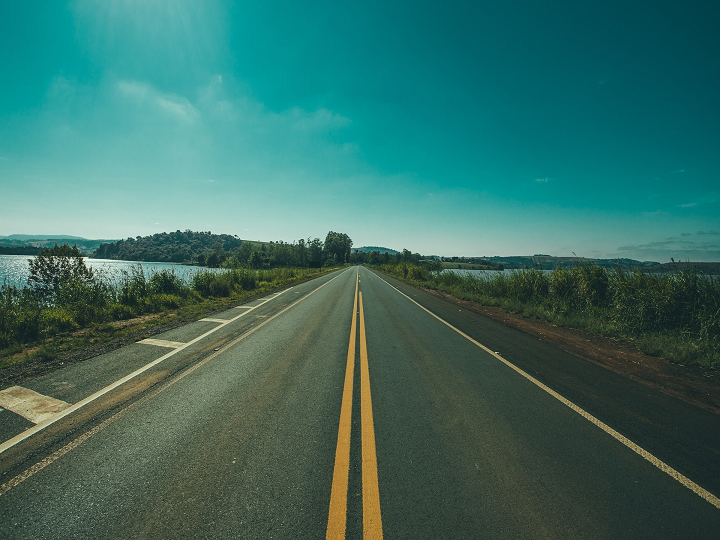
\includegraphics[width=\textwidth]{figures/fig_road.png}
	\caption{Original image.}
	\label{fig:road}
\end{minipage}
\hfill
\begin{minipage}[b]{0.32\textwidth}
	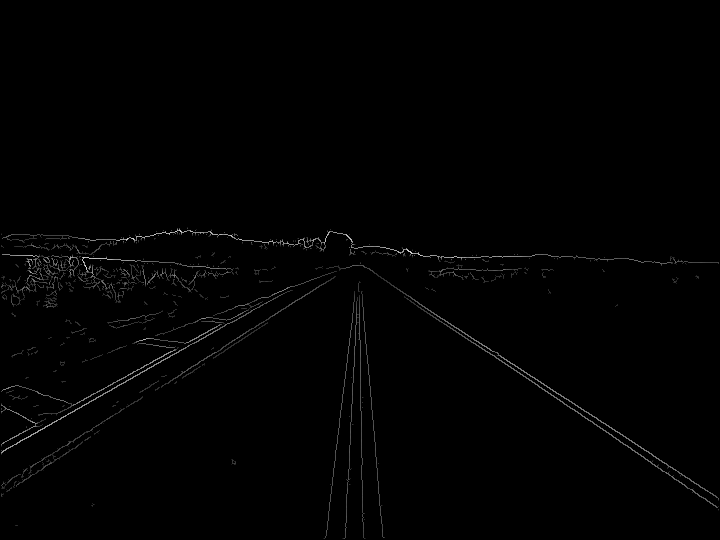
\includegraphics[width=\textwidth]{figures/fig_road_edges.png}
	\caption{Edge-detected image.}
	\label{fig:road_edges}
\end{minipage}
\hfill
\begin{minipage}[b]{0.32\textwidth}
	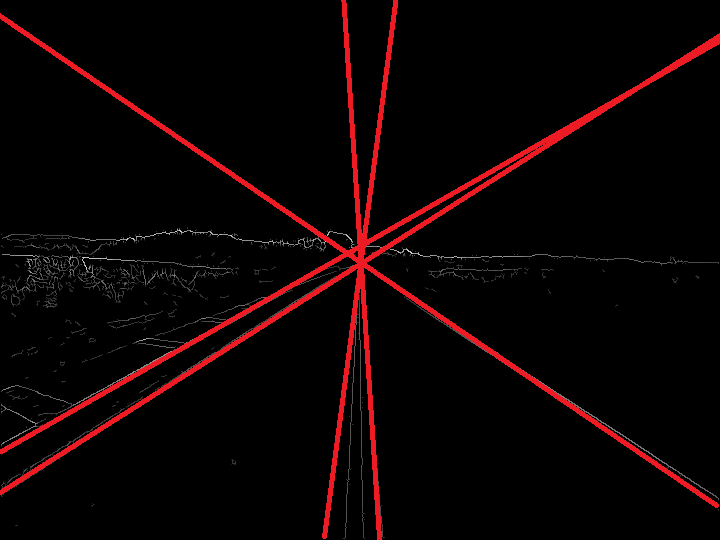
\includegraphics[width=\textwidth]{figures/fig_road_lines.png}
	\caption{Line-detected image.}
	\label{fig:road_lines}
\end{minipage}
\end{figure}




\section*{The Hesse Normal Representation for Lines}

Before starting our discussion of line detection, we must first consider the system we will use to describe lines in an image.
For efficiency, we want to describe a line using the fewest parameters possible. 
A commonly used line representation is $y = mx + b$ which describes lines using two parameters \textit{m} and \textit{b}.
The problem with this system is that it cannot describe vertical lines as m would assume an undefined value.
The line representation that we will use is known as the Hesse normal form. This system uses
two parameters ($\rho$, $\theta$) to describe a line \textbf{A} as follows:

\begin{enumerate}
\item $\rho$ is the distance from the origin (the center of the image) to the closest point on A.
\item $\theta$ is the angle between the x axis and the normal line connecting the origin to the closest point on A.
\end{enumerate}

To account for all possible lines in an image, the parameters range: $0 \leq \theta < 180^\circ$ and 

$-\sqrt(image\_height^2+image\_width^2)/2 \leq \rho \leq \sqrt(image\_height^2+image\_width^2)/2$

Examples of lines and their ($\rho$, $\theta$) parameters are shown in Figure~\ref{fig:hesse_normal_examples}.
The line being described is displayed in red, and the normal line is displayed in magenta. 
Take note that $\rho$ can be a negative value which extends the normal line in the reverse direction from the angle
denoted by $\theta$, as shown in Examples 2, 3, and 4. The line shown in Example 3 is
parameterized as $(-7, 0^\circ)$ and not $(7, 180^\circ)$, due to the valid range of theta: $0 \leq \theta < 180^\circ$.
For the same reason, the line in Example 4 is parameterized as $(-7, 90^\circ)$ and not $(7, 270^\circ)$.

\begin{figure}[H]
   \begin{center}
       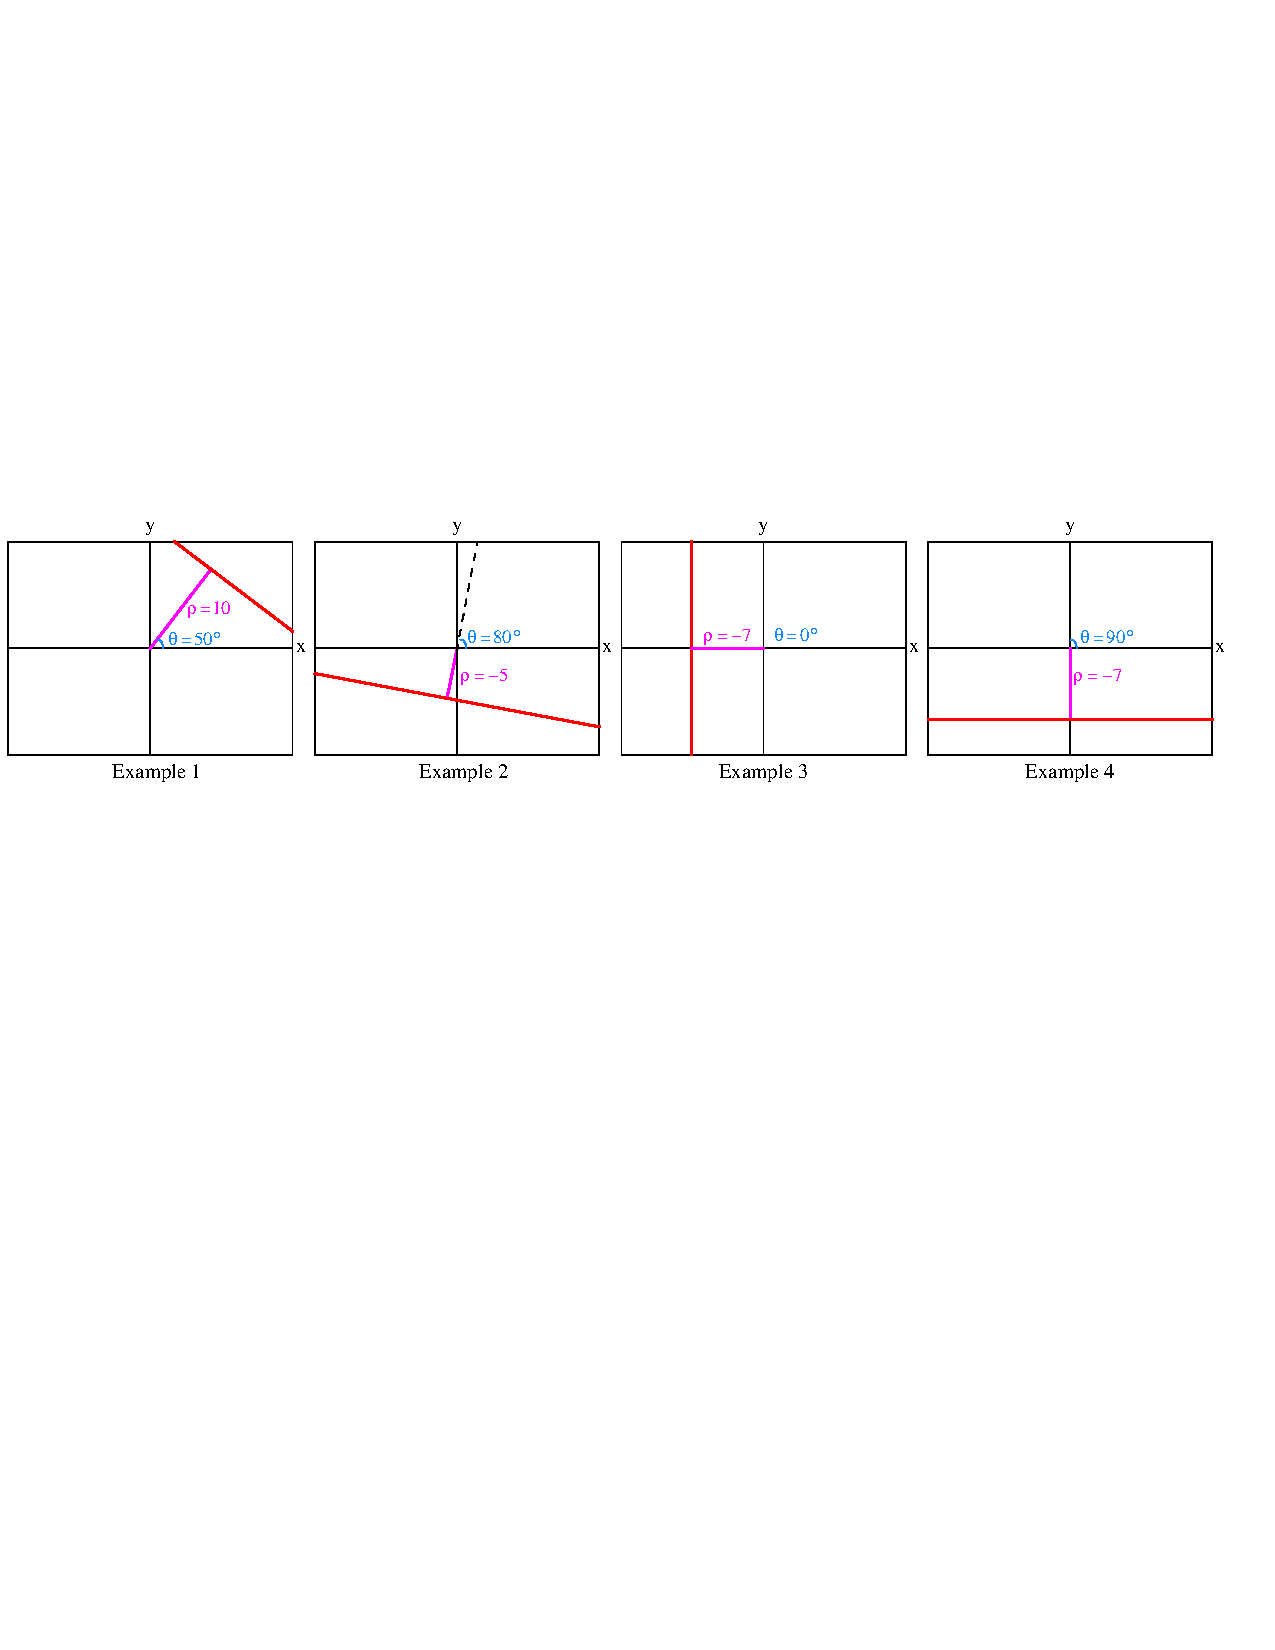
\includegraphics[scale = 0.78]{figures/fig_hesse_normal_examples}
   \end{center}
   \caption{Lines (in red) and their ($\rho$, $\theta$) parameters.}
	\label{fig:hesse_normal_examples}
\end{figure}

Lines described in ($\rho$, $\theta$) form can be mapped to pixels in (x,y) coordinates and vice-versa using the equation $\rho = x*cos(\theta) + y*sin(\theta)$. 
Note that a pixel can lie on an infinite number of lines, as there are the infinite $\theta$ values from $0^\circ$ to $180^\circ$.
Figure~\ref{fig:pixel_to_lines} shows a pixel at (x,y) coordinate (8,5) and some of the lines that it is positioned upon.

\begin{figure}[H]
   \begin{center}
       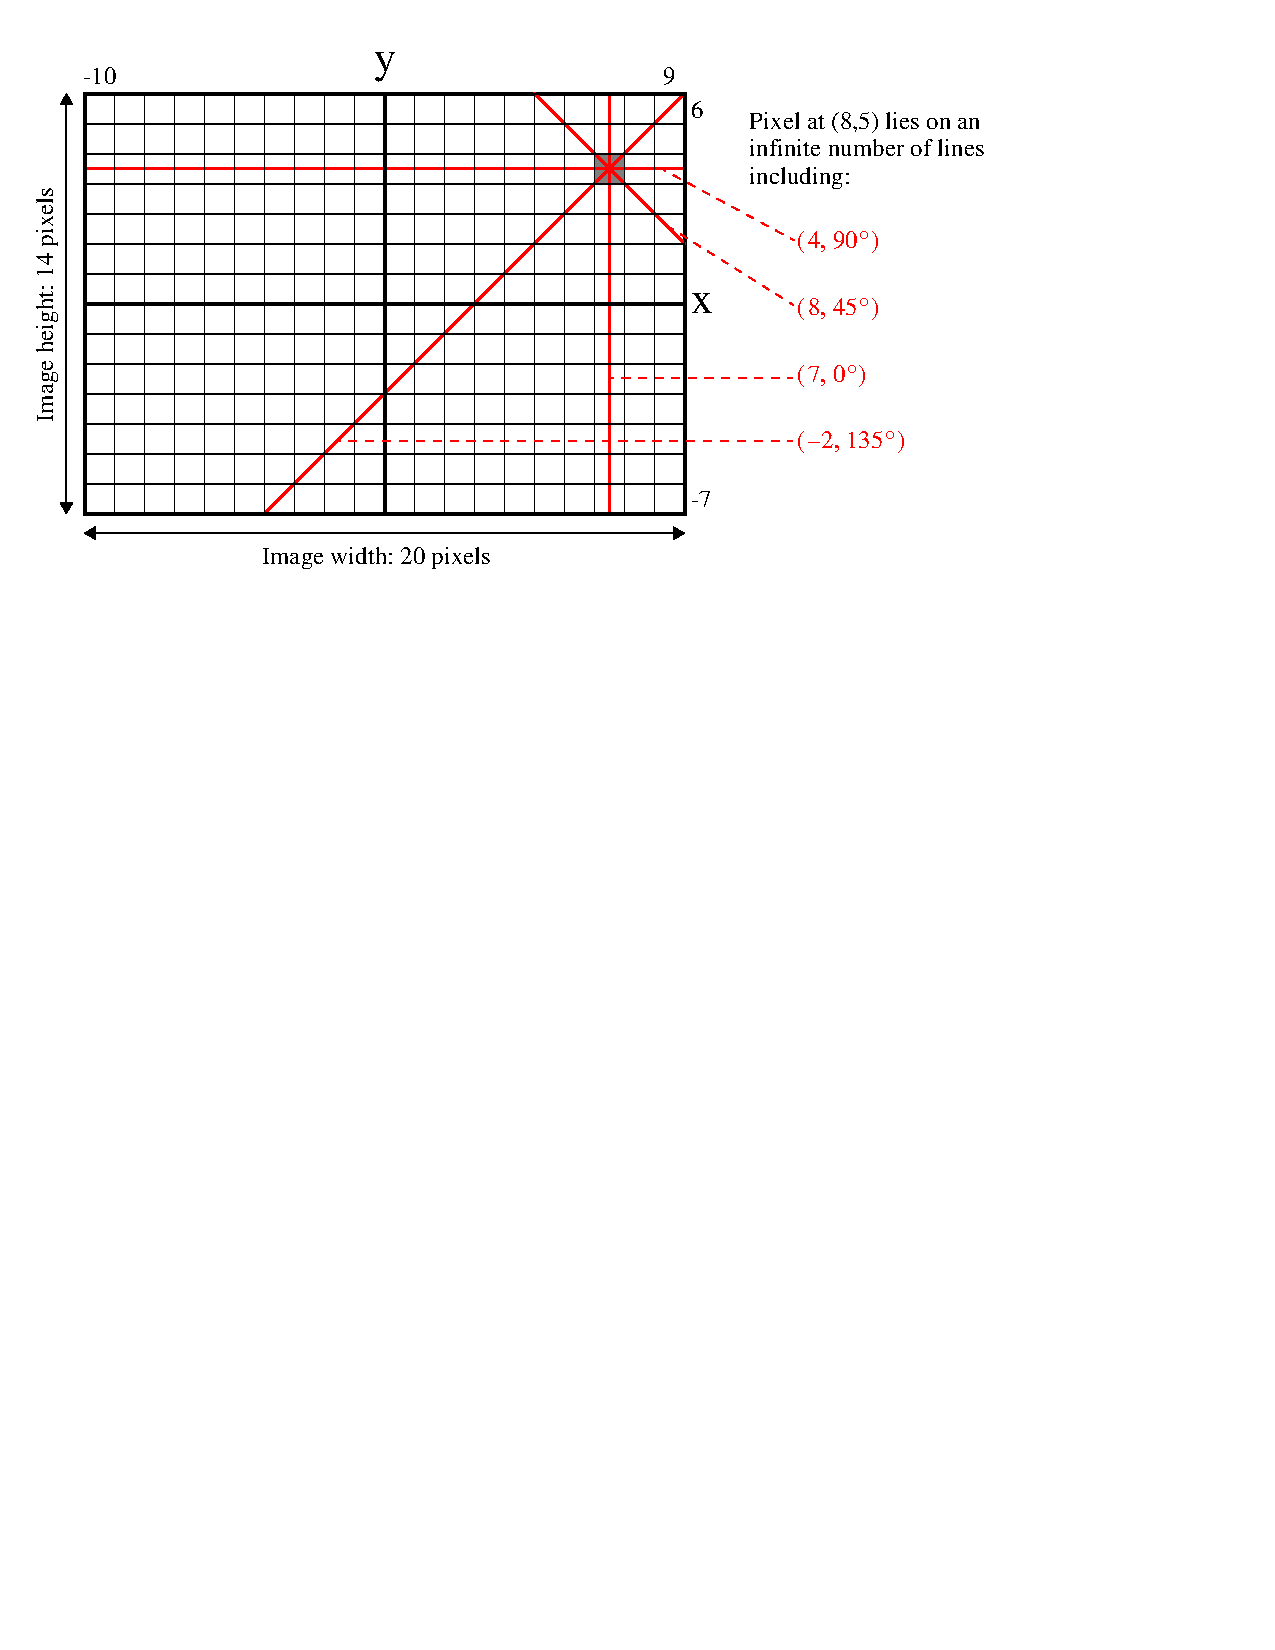
\includegraphics[scale = 0.95]{figures/fig_pixel_to_lines}
   \end{center}
   \caption{A pixel in an image can lie on an infinite number of lines, including the four lines shown.}
	\label{fig:pixel_to_lines}
\end{figure}


\pagebreak

\section*{The Hough Transform}

The Hough transform takes an edge-detected input image and transforms it to a 2-dimensional integer array called 
the accumulator.
The two dimensions of the accumulator are indexed by $\rho$ and $\theta$ respectively,
and each element stores how many edge pixels in the input image
are positioned along the corresponding line ($\rho$, $\theta$). 
%Effectively, the accumulator values measure the length of each line that is present in the input image. 
The most prominent lines in the input image can then be inferred by finding the lines with the 
highest values in the accumulator.
The process by which the Hough transform calculates the values in the accumulator is described below.

~\\
The accumulator elements are first initialized to zero, then \textit{accumulate} in value as the Hough transform
algorithm sweeps across the pixels of the input image. 
Each edge pixel encountered by the algorithm contributes +1 to the accumulator values
of all lines on which it is positioned. 
Since there are theoretically an infinite number of such lines, we must select a resolution for $\rho$ and $\theta$ to
limit the number of lines being tracked by the algorithm.

\begin{figure}[H]
   \begin{center}
       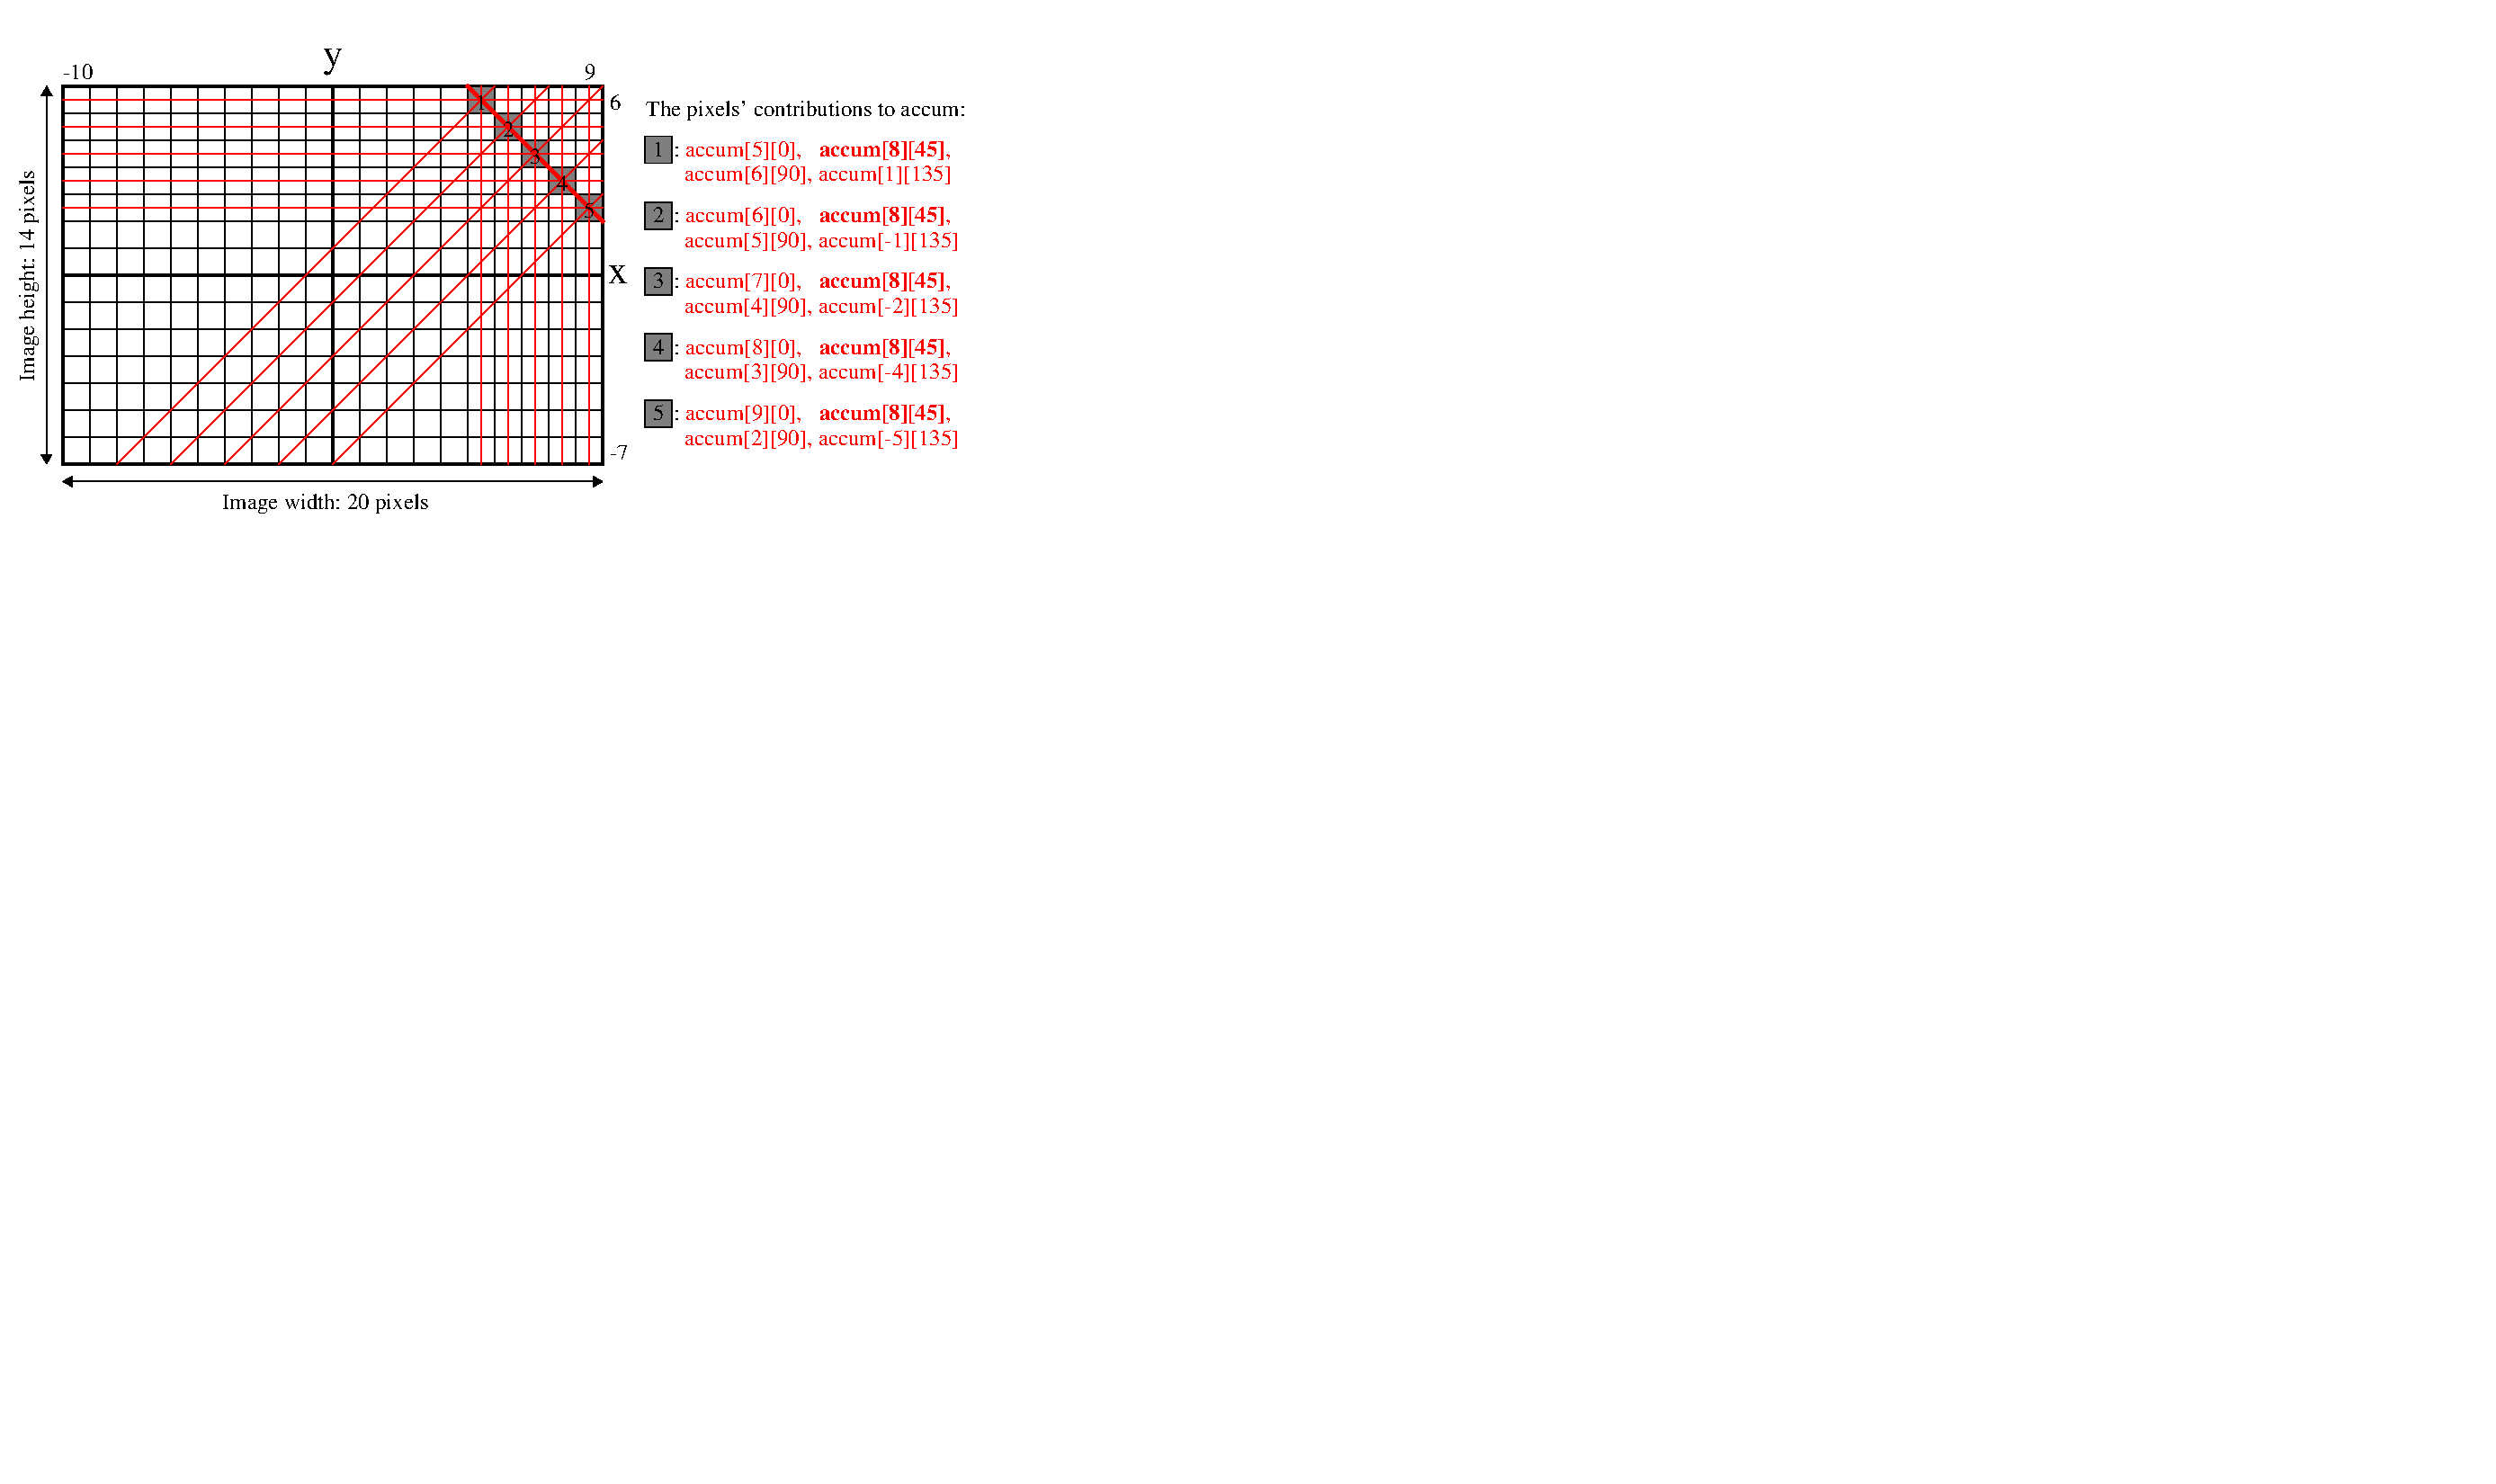
\includegraphics[scale = 0.83]{figures/fig_line_20x14}
   \end{center}
   \caption{Applying the Hough transform ($\theta$ resolution = $45^\circ$) on a 20x14 image with five edge pixels.}
	\label{fig:hough_demonstration}
\end{figure}

As a demonstration, let us choose a $\theta$ resolution of $45^\circ$ and a $\rho$ resolution of 1 pixel to 
transform a 20x14 image. This requires an accumulator array, \texttt{accum[RHOS][THETAS]}, with dimensions 
RHOS = 24, and THETAS = 4. Integer values of $\rho$ range $-12 \leq \rho < 12$, 
and $\theta$ values range $0^\circ, 45^\circ, 90^\circ,$ and $135^\circ$. 
Figure~\ref{fig:hough_demonstration} shows the operations involved in 
transforming a 20x14 edge-detected image with five edge pixels in the top-right corner. 
The five pixels form the line $(8, 45^\circ)$, which is shown as the bold red line.
Each pixel contributes +1 to the four accumulator indices corresponding to the four possible $\theta$ values.
The $\rho$ index corresponding to each $\theta$ is calculated using the formula $\rho = x*cos(\theta) + y*sin(\theta)$.
After the Hough transform completes, the accumulator is as shown in Figure~\ref{fig:accumulator}. As
expected, \texttt{accum[8][45$^\circ$]} has the highest value of 5, since there were five pixels along it in the input image.


\begin{figure}[H]
   \begin{center}
       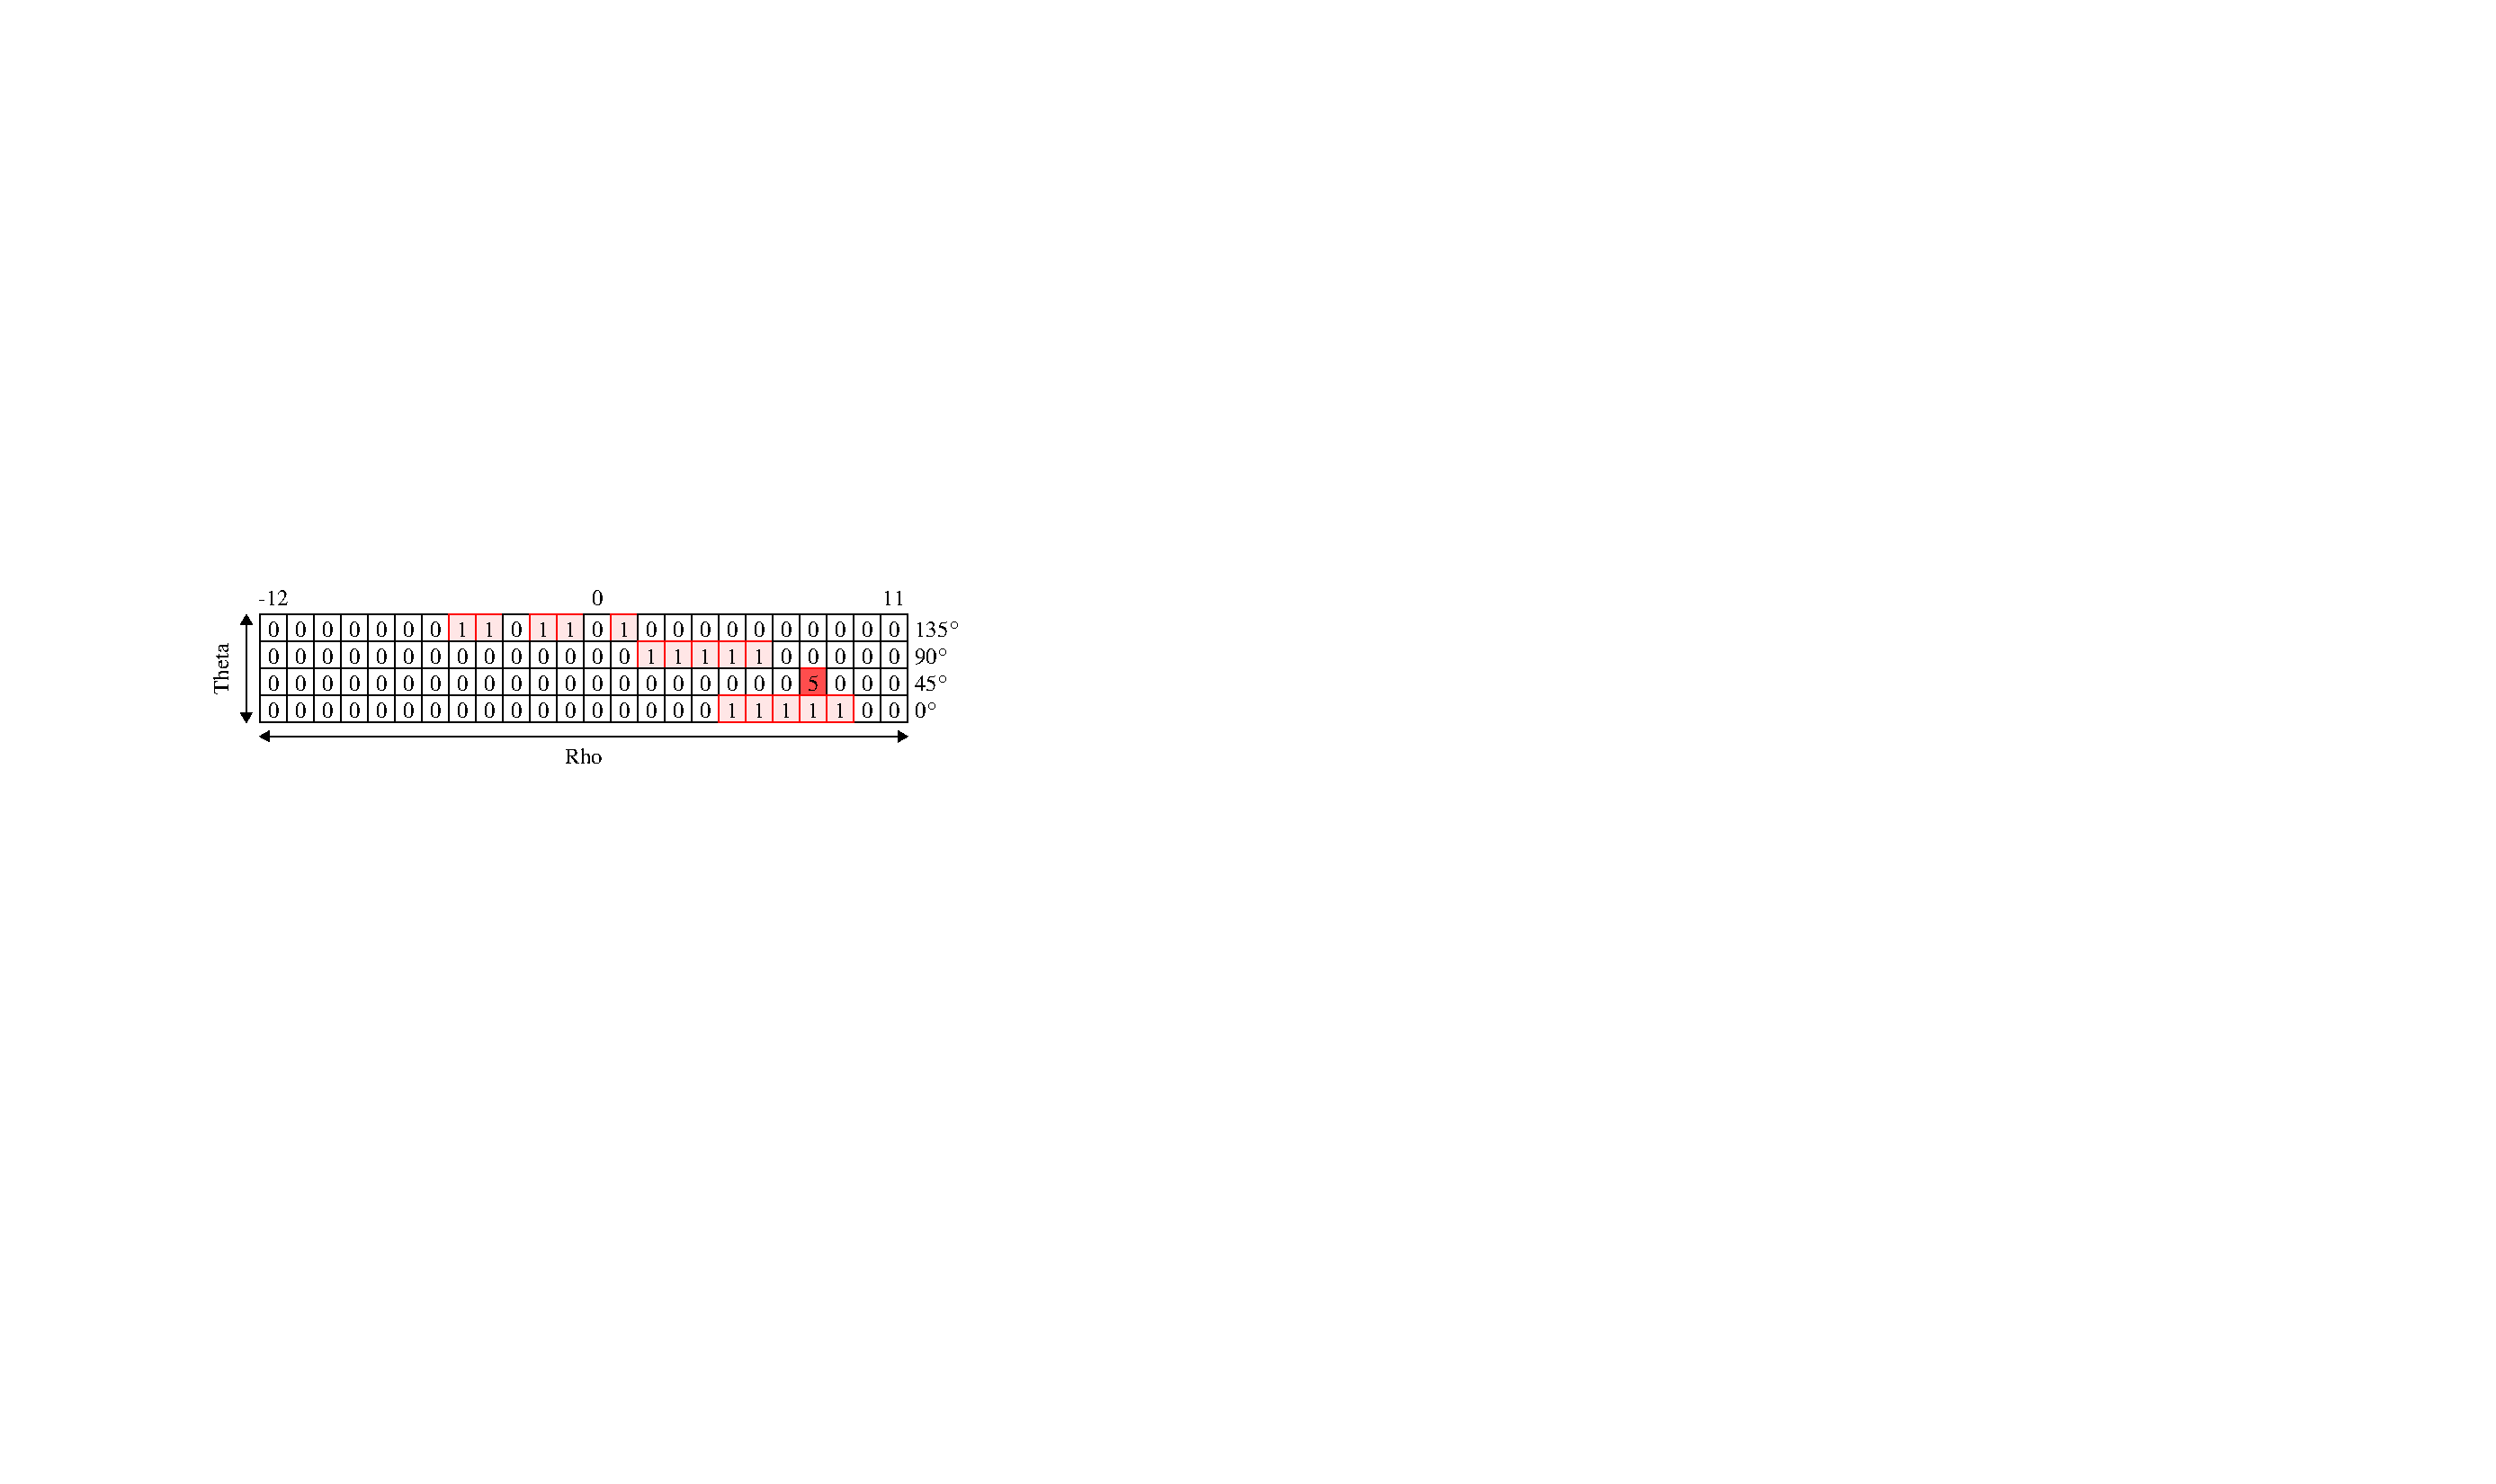
\includegraphics[scale = 0.8]{figures/fig_accumulator}
   \end{center}
   \caption{The accumulator resulting from the Hough transform of the image in Figure~\ref{fig:hough_demonstration}.}
	\label{fig:accumulator}
\end{figure}


\subsection*{Extracting Lines from Local Maxima in the Accumulator}


Upon completion of the Hough transform we are left with the task of extracting prominent lines from the accumulator.
The simplest method for extracting the N most prominent lines from the accumulator is to 
find the N highest values (global maxima). However, this approach is prone to issues which we will discuss below.

~\\
A source of error when using the Hough transform for line detection is the potential for  
the pixels of a single "real" line in an image contributing to multiple adjacent elements in 
the accumulator. This could happen if the line was not perfectly straight due to noise, or if 
our resolution for $\rho$ or $\theta$ was inadequate. For example, consider transforming an image with the line 
(11,$7.5^\circ$) using a $\theta$ resolution of $1^\circ$. During the transform some of the pixels in the line may
contribute to \texttt{accum[11][7]} while others may contribute to \texttt{accum[11][8]} resulting in
multiple nearby accumulator elements with similarly high values.
After the transform if we simply searched for the global maxima to detect lines,
we could falsely detect two or more lines resulting from the single real line.

~\\
To eliminate false duplicates, we will extract lines from local maxima in the accumulator rather than global maxima.
Whenever there are multiple high accumulator values in a vicinity we will only consider the one whose 
value is highest, and eliminate those neighboring. This approach allows us to detect the single line which is likely the best
fit to the real line in the input image. 
Figures~\ref{fig:global_maxima} and \ref{fig:local_maxima} illustrate the differences between global maxima and
local maxima extraction. Note that this approach runs the risk of elliminating lines that actually did exist near eachother
in the input image, but for the purposes of lane detection we can assume lane markings are sufficiently spaced apart for
this to not be an issue.

~\\
Searching for local minima also allows us to search for a fewer lines in total while cover all of the lanes in the image. 
Consider an image with two lane markings where one was significantly longer than the other. In this case,
the longer lane may yield multiple accumulator values that are greater than any of the values
for the shorter lane. If we then searched for two global maxima with the expectation of detecting the two lanes, 
we would detect the longer lane twice and the shorter lane not at all. Searching for local maxima means that we would
only extract one line corresponding to the longer lane, allowing for the detection of the second lane as long as it was the
second highest local maximum in the accumulator.


\begin{figure}[h]
\centering
\begin{minipage}[b]{0.47\textwidth}
	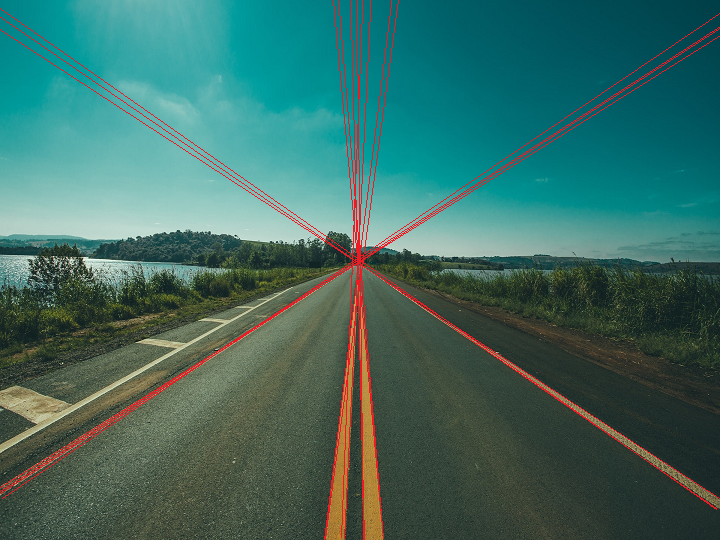
\includegraphics[width=\textwidth]{figures/fig_road_lines_global_maxima.png}
	\caption{Lines extracted from global maxima.}
	\label{fig:global_maxima}
\end{minipage}
\hfill
\begin{minipage}[b]{0.47\textwidth}
	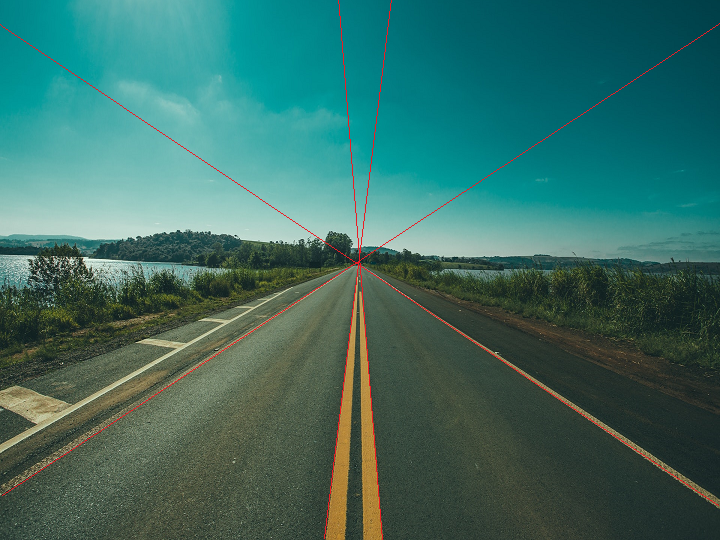
\includegraphics[width=\textwidth]{figures/fig_road_lines_local_maxima.png}
	\caption{Lines extracted from local maxima.}
	\label{fig:local_maxima}
\end{minipage}
\end{figure}

\subsection*{Elliminating the Horizon and Horizontal Lines}

To improve the accuracy of our lane detector, we will make two simple optimizations to the Hough transform and
line extraction.

~\\
The first optimization aims to prevent detecting lines from objects far in the horizon (such as those detected from hills or clouds). Figure~\ref{fig:local_maxima} shows an example where the upper portion of the image contains the horizon and
the sky. When implementing the Hough transform we will elliminate the horizon by 
only going through the bottom half of the edge-detected image when incrementing the accumulator.
%limiting the Y coordinate range of pixels that we sweep through the pixels of the input image during the Hough transform.
Not only will this optimization potentially prevent false lines, it will reduce the runtime of the Hough transform by
skipping over half of the input pixels.

~\\
The second optimization elliminates horizontal lines from being extracted from the accumulator. 
This optimization is based on the knowledge that lanes boundaries 
will tend to point outward from the camera's perspective (from the bottom of the image towards the top), 
meaning that vertical and slanted lines are the ones likely to correspond to lanes. 
Figure~\ref{fig:bus} shows a scenario where this optimization is particularly beneficial, as the merging bus contains features
that would result in prominent horizontal lines being detected. 
We can implement this optimization in our line extraction stage by ignoring the lines in the accumulator whose $\theta$
indicates a horizontal line ($80^\circ < \theta < 100^\circ$). 

\begin{figure}[H]
   \begin{center}
       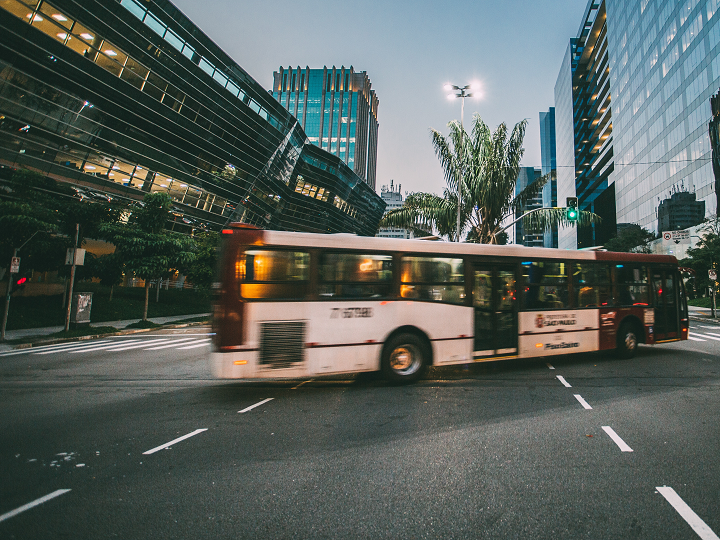
\includegraphics[scale = 0.3]{figures/fig_bus}
   \end{center}
   \caption{A merging bus contains prominent horizontal lines that may be detected instead of the lane markings.}
	\label{fig:bus}
\end{figure}


\section*{Part 1}

Write a C-language program to implement the Hough transform. 
Start with the skeleton code provided in \textit{/design\_files/part1/hough.c}. 
Your program should load a 720x540 BMP image, apply edge detection, apply the Hough transform, extract the lines, 
overlay the lines onto the original image, then save the resulting image as a BMP file. 

~\\
Your Hough transform should use a $\theta$ resolution of $1^\circ$ and a $\rho$ resolution of 2 pixels. 
Ellminate the horizon and horizontal lines using the optimizations described in the previous section.
Extract five lines from the five highest local maxima in the accumulator. 
A value is considered the local maximum if it is the highest value in the 5x5 square around it (+/- 2 to the $\rho$ and $\theta$ indices). 
Overlay the extracted lines onto the original image (as shown in Figure~\ref{fig:local_maxima}), then save it as a BMP file. 
Use the images provided in \textit{/design\_files/test\_images/} to test your program.
How closely do the detected lines align to the lane boundaries? For images
where lane detection was less successful, explain potential source(s) of error.

~\\
Record the runtime of the Hough transform across the test images.
Why does the Hough transform runtime vary by image?
Using the average total runtime across the images, calculate framerate at which you processed them.
The total runtime includes edge detection, Hough transform, and line extraction, but not operations
involved with loading and saving the BMP images.
Determine the upper bound on the runtime of the Hough transform and calculate the minimum framerate.


\section*{Part 2}

Create an OpenCL kernel for the Hough transform. Start with the
the skeleton code provided in \textit{/design\_files/part2/}. 
Use the same parameters as in Part 1.
To improve performance, use local memory to hold the accumulator array and unroll critical loop(s).
Instantiate your edge detection kernel from Exercise 2 to compile a single \textit{.aocx} image that 
contains both the edge detector and the hough transform.

~\\
Skeleton host code is provided in \textit{/design\_files/part2/host/}. You must add to the code so that
the host program first calls the edge detection kernel, waits for it to complete, then feeds the edge detected data
buffer to the hough transform kernel. As in Part 1, your host program should extract five lines from the five 
highest local maxima in the accumulator, overlay them onto the original image, and save it as a BMP file.

~\\
Record the runtime of the Hough transform across the test images. How does the runtime compare to your
implementation in Part 1? Using the average total runtime across the images, calculate framerate at which you processed them.
Determine the upper bound on the runtime of the Hough transform and calculate the minimum framerate.

~\\
When implementing the Hough transform kernel, you can use the pragma \texttt{\#pragma ivdep}
to tell the OpenCL compiler that accesses to \texttt{accum} in subsequent loop iterations are free of data dependencies for
better pipelining of the circuit.
The OpenCL compiler would otherwise have difficulty in determining the lack of dependency, as subsequent indices calculated by
the formula $\rho = x*cos(\theta) + y*sin(\theta)$ are seemingly unpredictable.
We as designers however, know that the formula will ensure subsequent accesses to \texttt{accum} will be at different indices,
as we sweep $\theta$ from $0^\circ$ to $179^\circ$ for each edge pixel.

\section*{Part 3}

Improve the performance of your design from Part 2 by using OpenCL pipes to connect the output of your edge-detection kernel 
to the input of your Hough transform kernel. Doing this allows your kernels to share data completely inside the FPGA,
rather than using slow external memory as intermediary storage. Use a blocking pipe with a depth of 1.
Compile your piped kernels using the \texttt{aoc} flag \texttt{-profile=all} to enable profiling.
Make the necessary modifications to your host program to support your newly piped kernels. 

~\\
After running your application, use the profile monitor to check for kernel stalls.
Do your kernels stall as a result of the blocking pipe? What do the stalls (or lack of stalls)
indicate about the throughput of your edge detection kernel compared to your Hough transform kernel?

~\\
Record the runtime of your piped implemention across the test images. How does the runtime compare to your
implementation in Part 2? Using the average total runtime across the images, calculate framerate at which you processed them.
Determine the upper bound on the runtime of the Hough transform and calculate the minimum framerate.


%%%%%%%%%%%%%%%%%%%%%%%%%%%%%%%%%%%%%%%%
%%% FPGAcademy Copyright Information %%%
%%%%%%%%%%%%%%%%%%%%%%%%%%%%%%%%%%%%%%%%

%Always put the copyright on a new page (clear page), with some vertical space from top
\clearpage
\vspace{1in}

\noindent

Copyright {\copyright} FPGAcademy.org. All rights reserved. FPGAcademy and the 
FPGAcademy logo are trademarks of FPGAcademy.org.  This document is provided 
"as is", without warranty of any kind, express or implied, including but not 
limited to the warranties of merchantability, fitness for a particular purpose 
and noninfringement. In no event shall the authors or copyright holders be 
liable for any claim, damages or other liability, whether in an action of 
contract, tort or otherwise, arising from, out of or in connection with the 
document or the use or other dealings in the document.
~\\
~\\
**Other names and brands may be claimed as the property of others.


\end{document}
